\section{Datos, reproducción y estado de las afirmaciones}\label{sec:datos}
Esta sección reúne los datos que acompañan al artículo, explica cómo repetir los cálculos y
precisa qué tipo de evidencia respalda cada afirmación.

\subsection{Contraste con los conteos exactos}
En los tamaños estudiados, $Q(n)$ se conoce exactamente~\cite{oeis,q27}. La
Figura~\ref{fig:counts} muestra $nR_Q(n)$ para $16\le n\le27$, calculado tomando el logaritmo
del conteo entero y restando, antes de multiplicar por $n$, el logaritmo numérico del predictor.
En estos doce tamaños se observa una oscilación de periodo cuatro. Un ajuste con $\cerr$ prefijado
y una corrección $a/n$ describe parte de la variación (Apéndice~\ref{app:numquad}). Estos datos
son compatibles con la estimación de $\cerr$. Los conteos y los valores del predictor están en
\texttt{suplemento/datos/c\_n.json}.
\begin{figure}[ht]
\centering
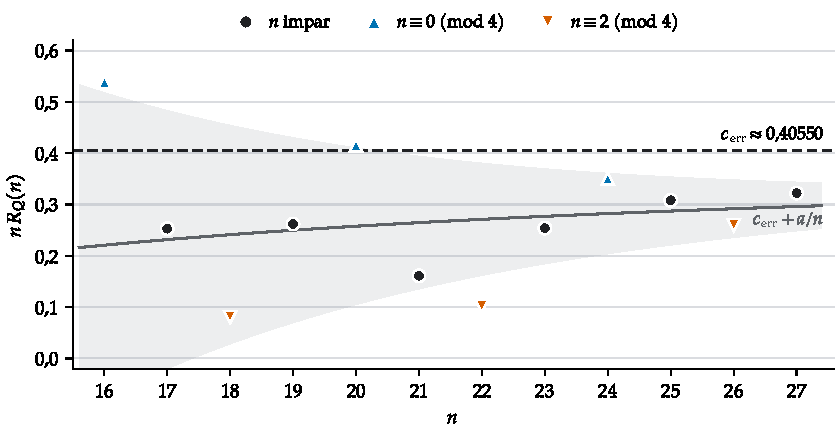
\includegraphics[width=.9\linewidth]{figuras/conteos.pdf}
\caption{Valores de $nR_Q(n)$ para $16\le n\le27$, obtenidos de los conteos exactos y del predictor
canónico (evidencia numérica). La línea discontinua marca el valor de $\cerr$ obtenido del continuo
y fijado antes del ajuste a estos doce tamaños. La curva gris
muestra la deriva ajustada $\cerr+a/n$, con $a\simeq-2{,}956$, y la banda sombreada tiene la amplitud
$Ae^{-\kappa(n-16)}$ de la oscilación de periodo cuatro (Apéndice~\ref{app:numquad}). Los tamaños
impares tienen oscilación ajustada cero. En los tamaños pares el modelo suma esa amplitud
si $n\equiv0\;(\mathrm{mod}\,4)$ y la resta si $n\equiv2\;(\mathrm{mod}\,4)$.}\label{fig:counts}
\end{figure}


\subsection{Reproducción del valor numérico}
El suplemento contiene las mallas finales, los programas de análisis, los valores en los nodos,
los intervalos y las huellas SHA256 de todos los archivos.
Con Python~3 y NumPy, la orden \texttt{python -B replica/reproducir\_valor.py replay}, ejecutada
desde \texttt{suplemento}, rehace el análisis en un directorio nuevo y debe dar $0{,}4055003786$ a
diez decimales. La guía del suplemento explica también cómo regenerar las mallas desde el principio.
La ejecución principal constó de 955 tareas y tardó 168,3 minutos con 16 procesos; la
complementaria, de 132 tareas y 30,1 minutos.

\subsection{Certificados por intervalos}
En \texttt{suplemento/certificados} están los programas que generan los intervalos del perfil, de
$S$, de $P_T$ y de $Q_2$ en el décimo nodo de la regla de Gauss--Legendre de veinte puntos, junto
con el núcleo bivariante con signo de ese nodo y una prueba rápida de las entradas. Cada
certificado registra la precisión empleada, sus entradas y el intervalo obtenido; la
Sección~\ref{sec:numcert} explica qué se certifica y hasta dónde.

\subsection{Predicciones registradas}
En las comprobaciones con tableros finitos, la predicción, los casos y la regla de comparación se
fijaron antes de evaluar, en un archivo con marca de tiempo y huella SHA256. El estudio del
cuadrado, por ejemplo, registró once predicciones: ocho en casos ciegos y tres en controles
conocidos.
